\documentclass[tikz, border=2pt]{standalone}
\usepackage{amsmath}

\begin{document}
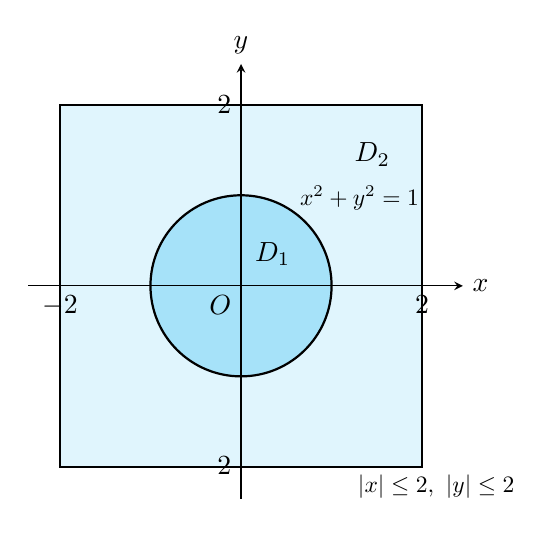
\begin{tikzpicture}[scale=1.15, >=stealth]
    % Rectangle |x|<=2, |y|<=2 split by the unit circle.
    \fill[cyan!12] (-2,-2) rectangle (2,2);
    \fill[cyan!35] (0,0) circle (1);

    \draw[->] (-2.35,0) -- (2.45,0) node[right] {$x$};
    \draw[->] (0,-2.35) -- (0,2.45) node[above] {$y$};

    \draw[thick] (-2,-2) rectangle (2,2);
    \draw[thick] (0,0) circle (1);

    \draw[dashed] (-2,0) node[below] {$-2$} -- (-2,2);
    \draw[dashed] (2,0) node[below] {$2$} -- (2,2);
    \draw[dashed] (0,2) node[left] {$2$} -- (2,2);
    \draw[dashed] (0,-2) node[left] {$-2$} -- (2,-2);

    \node[below left] at (0,0) {$O$};
    \node at (0.35,0.35) {$D_1$};
    \node at (1.45,1.45) {$D_2$};
    \node[above right, scale=0.85] at (0.56,0.75) {$x^2+y^2=1$};
    \node[below right, scale=0.85] at (1.2,-2) {$|x|\leq2,\ |y|\leq2$};
\end{tikzpicture}
\end{document}
